\section{Zielsetzung}
\label{sec:Zielsetzung}
Es soll die Suszeptibilität paramgnetischer Stoffe bestimmt werden. Dies wird durch eine Brückenschaltung für
drei verschiedene seltene Erden realisiert.

\section{Theorie}
\label{sec:Theorie}
Die magnetische Flussdichte $\vec{B}$ und die magnetische Feldstärke $\vec{H}$ hängen in Materie durch die
Beziehung
\begin{equation}
    \vec{B} = \mu_{0}\vec{H}+\vec{M}
\end{equation}
ab. Dabei ist $\vec{M}$ die Magnetisierung und $\mu_{0}$ die magnetische Feldkonstante. $\vec{M}$ hängt von
$\vec{H}$ durch die Suszeptibilität $\chi$ durch
\begin{equation}
    \vec{M} = \mu_{0}\chi\vec{H}
\end{equation}
ab. $\chi$ ist dabei keineswegs eine Konstante, sondern hängt in komplizierter Weise von $\vec{H}$ und der
Temperatur $T$ ab. Allgemein tritt für alle Atome der Diamagnetismus auf, da er durch ein von außen angelegtes
Magnetfeld magnetische Momente im Atom induziert, so dass ein dem äußeren entgegengestztes Magnetfeld induziert
wird. In diesem Fall ist $\chi < 0$. Im Gegensatz dazu tritt der Paramagnetismus nur bei Atomen, Molekülen oder
Ionen auf, die keinen verschwindenden Gesamtdrehimpuls $\vec{J}$ haben. Er entsteht dadurch, dass sich die mit
dem Drehimpuls gekoppelten magnetischen Momente relativ zum äußeren Magnetfeld ausrichten. Da die magnetischen
Momente durchgängig durch die thermische Bewegung gestört werden, ist der Paramagnetismus temperaturabhängig.
Für den Diamagnetismus trifft dies nicht zu. Der Gesamtdrehimpuls setzt sich aus dem Bahndrehimpuls $\vec{L}$
und dem Spin $\vec{S}$ durch
\begin{equation}
    \vec{J} = \vec{L} + \vec{S}
\end{equation}
zusammen. Die magnetischen Momente zum Drehimpuls und Spin ergeben sich zu
\begin{equation}
    \vec{\mu}_{\symup{L}} = -\frac{\mu_{\symup{B}}}{\hbar} \vec{L}
\end{equation}
und
\begin{equation}
    \vec{\mu_{\symup{S}}} =  -g_{\symup{S}}\frac{\mu_{\symup{B}}}{\hbar}\vec{S}\,.
\end{equation}
$\hbar$ ist dabei das reduzierte Plancksche Wirkungsquantum, $\mu_{\symup{B}}=\frac{e_{0}\hbar}{2m_{0}}$ das
Bohrsche Magneton und $g_{\symup{S}}$ das gyromagnetische Verhältnis des freien Elektrons.
\begin{figure}
    \centering
    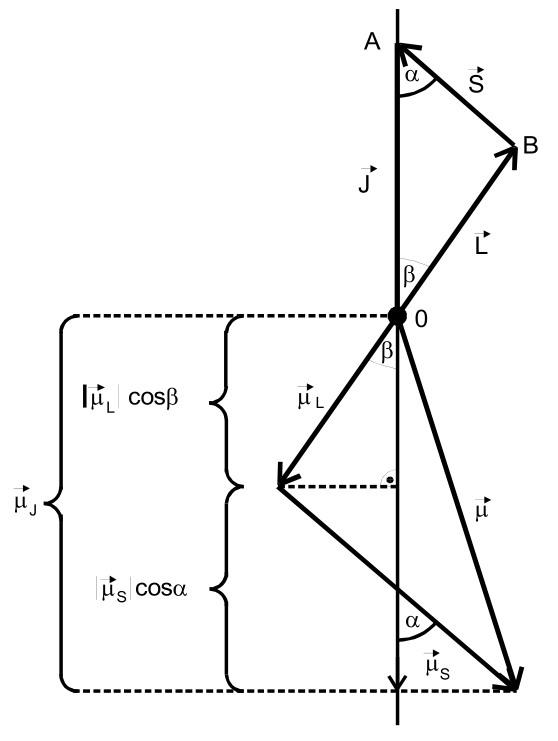
\includegraphics[width=0.4\textwidth]{bilder/vektordiagramm.png}
    \caption{Vektordiagramm der Drehimpulsvektoren und den magnetischen Momenten \cite{sample}.}
    \label{fig:vektordiagramm}
\end{figure}
Aus den geometrischen Zusammenhänge aus \autoref{fig:vektordiagramm} ergibt sich
\begin{equation}
    |\vec{\mu_{\symup{J}}}| = |\vec{\mu_{\symup{S}}}|\cos{\alpha}| + |\vec{\mu_{\symup{L}}}|\cos{\beta}
\end{equation}
Weiterhin gelten für $|\vec{\mu_{\symup{L}}}|$ und $|\vec{\mu_{\symup{S}}}|$
\begin{align*}
    |\vec{\mu_{\symup{L}}}| &= \mu_{\symup{B}}\sqrt{L\left(L+1\right)} \\
    |\vec{\mu_{\symup{S}}}| &= g_{\symup{S}}\mu_{\symup{B}}\sqrt{S\left(S+1\right)}\,.
\end{align*}
Mit Hilfe des durch
\begin{equation*}
    g_{\symup{J}} = \frac{3J\left(J+1\right) + S\left(S+1\right)- L\left(L+1\right)}{2J\left(J+1\right)}
\end{equation*}
definierten Lande-Faktors ergibt sich dann
\begin{equation}
    |\vec{\mu_{\symup{J}}}| \approx \mu_{\symup{B}}g_{\symup{J}}\sqrt{J\left(J+1\right)}\,.
\end{equation}